\chapter{Testes sintéticos para o cálculo das componentes e da amplitude do vetor magnético}
\label{chap:synt_tests_II}

Testamos a técnica da camada equivalente para o cálculo das componentes e da amplitude do vetor magnético em dois conjuntos de dados sintéticos simulando diferentes amostras de rochas. No primeiro teste, aplicamos a técnica para analisar a dependência da direção de magnetização para o cálculo das componentes e da amplitude em um modelo que representa uma amostra de rocha homogeneamente magnetizada (Seção \ref{sec:simple_sample}). No segundo, o conjunto de dados sintéticos é gerado por um modelo com mais complexidade que contém grãos fortemente magnetizados e concentrados em uma determinada região ao longo da amostra sintética de rocha (Seção \ref{sec:hetero_sample}). 

\section{Simulação de amostra simples}
\label{sec:simple_sample}

Geramos uma amostra de rocha sintética que pode simular tanto uma rocha ígnea quanto uma rocha sedimentar com intensidade de magnetização alta, considerando que a mesma seja homogeneamente magnetizada \citep{collinson1983,dunlop1997}. Com este propósito, geramos um prisma retangular de dimensões $18$ mm, $12$ mm e $2$ mm ao longo dos eixos $x$, $y$ e $z$, respectivamente. A intensidade de magnetização é igual a $1,5$ A/m. A direção de magnetização é $20^\circ$ para a inclinação e $30^\circ$ para a declinação. Os dados foram calculados em um grid regular de $100 \times 100$ pontos ao longo dos eixos $x$ e $y$, respectivamente. A distância sensor-amostra simulada foi fixada em $150$ microns acima da superfície da amostra. Por fim, os dados foram contaminados com ruído Gaussiano de média zero e desvio padrão $20$ nT. A componente vertical do campo magnético pode ser vista na figura \ref{fig:bz_homo_sample}.       

%%% Figuras teste 1
\begin{figure}
	\centering
	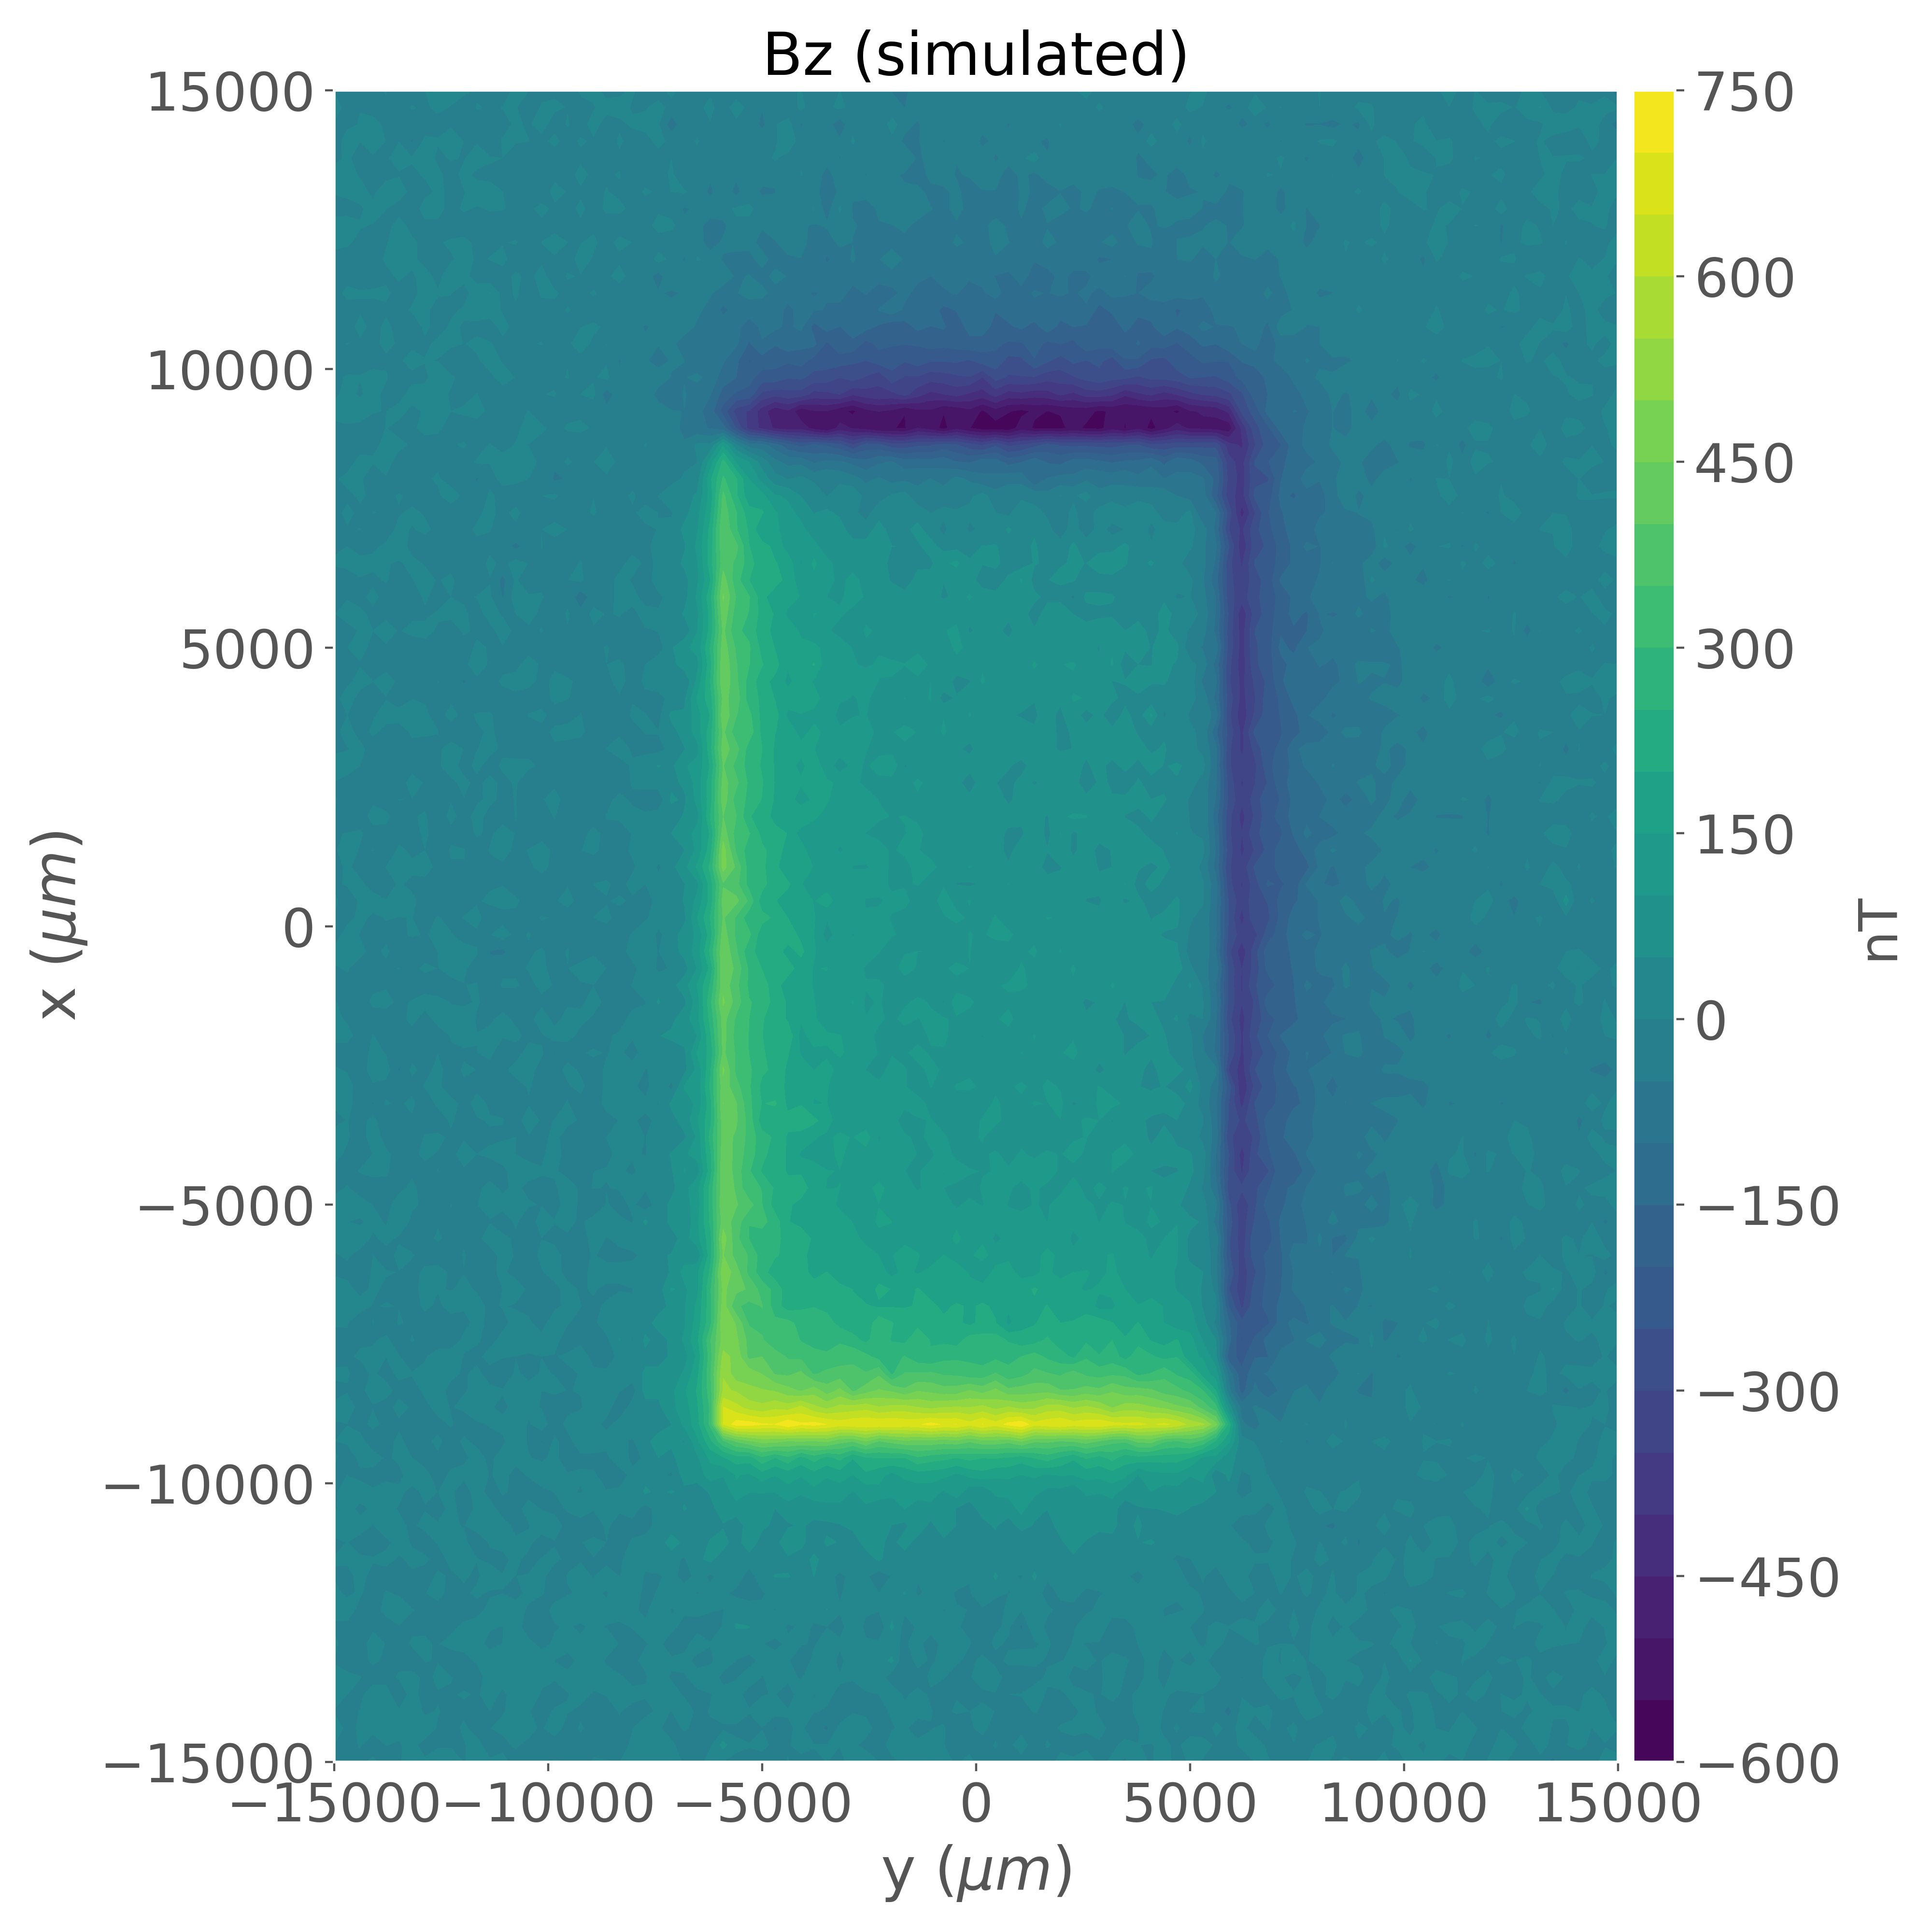
\includegraphics[width=.9\textwidth]{Fig/mag_vec/amostra_homo_correto/noisy_bz_sample.png}
	\caption{Aplicação a dados sintéticos para amostra homogeneament magnetizada. Componente vertical do campo magnético observado contaminada com ruído Gaussiano de média zero e desvio padrão $20$ nT. A direção de magnetização é igual a $20^\circ$ para a inclinação e $30^\circ$ para a declinação. A distância sensor-amostra igual a $150$ microns. }
	\label{fig:bz_homo_sample}
\end{figure}

\subsection{Camada equivalente com a mesma direção de magnetização da amostra}
\label{subsec:homo_same_dir}

Utilizamos uma camada equivalente composta por um grid de $100 \times 100$ posicionados a uma profundidade de $z_c = 750$ microns abaixo do plano de observação. A direção de magnetização para as fontes equivalente foi de $20^\circ$ para a inclinação e $30^\circ$ para a declinação. Utilizando a equação \ref{eq:linear_sys_p_z}, estimamos a distribuição de momentos magnéticos (não mostrado). A figura \ref{fig:datafit_homo_sample_samedir}b mostra os dados preditos produzidos pela camada equivalente. A figura \ref{fig:datafit_homo_sample_samedir}c mostra os resíduos definidos pela diferença entre os dados simulados (Figura \ref{fig:datafit_homo_sample_samedir}a) e os dados preditos (Figura \ref{fig:datafit_homo_sample_samedir}b). Os resíduos aparecem com distribuição normal de média $-0,02 \, nT$ e desvio padrão $14,36 \, nT$ como mostrado na figura \ref{fig:datafit_homo_sample_samedir}d. Com a distribuição de momentos magnéticos estimada, conseguimos calcular as componentes e a amplitude do campo magnético através das equações \ref{eq:pred_vec_x}, \ref{eq:pred_vec_y} e \ref{eq:amplitude_field} (Figura \ref{fig:components_homo_sample_samedir}a-d). Com o objetivo de verificarmos se a camada equivalente produziu as componentes e a ampĺitude do campo magnético com sucesso, calculamos os valores verdadeiros que são mostrados nas  figuras \ref{fig:comparison_homo_sample_samedir}a, \ref{fig:comparison_homo_sample_samedir}e e \ref{fig:comparison_homo_sample_samedir}i. As figuras \ref{fig:comparison_homo_sample_samedir}b, \ref{fig:comparison_homo_sample_samedir}f e \ref{fig:comparison_homo_sample_samedir}j são os dados preditos pela camada equivalente. As figuras \ref{fig:comparison_homo_sample_samedir}c, \ref{fig:comparison_homo_sample_samedir}g e \ref{fig:comparison_homo_sample_samedir}k são resíduos entre os dados verdadeiros e os dados preditos pela camada. As figuras \ref{fig:comparison_homo_sample_samedir}d, \ref{fig:comparison_homo_sample_samedir}h e \ref{fig:comparison_homo_sample_samedir}l são os histogramas dos resíduos. Diante destes resultados, podemos concluir que as estimativas para as componentes e a amplitude do campo magnético foram aceitáveis, de forma que a inversão produziu dados muito próximos dos verdadeiros.  

%% Figuras 

\begin{figure}
	\centering
	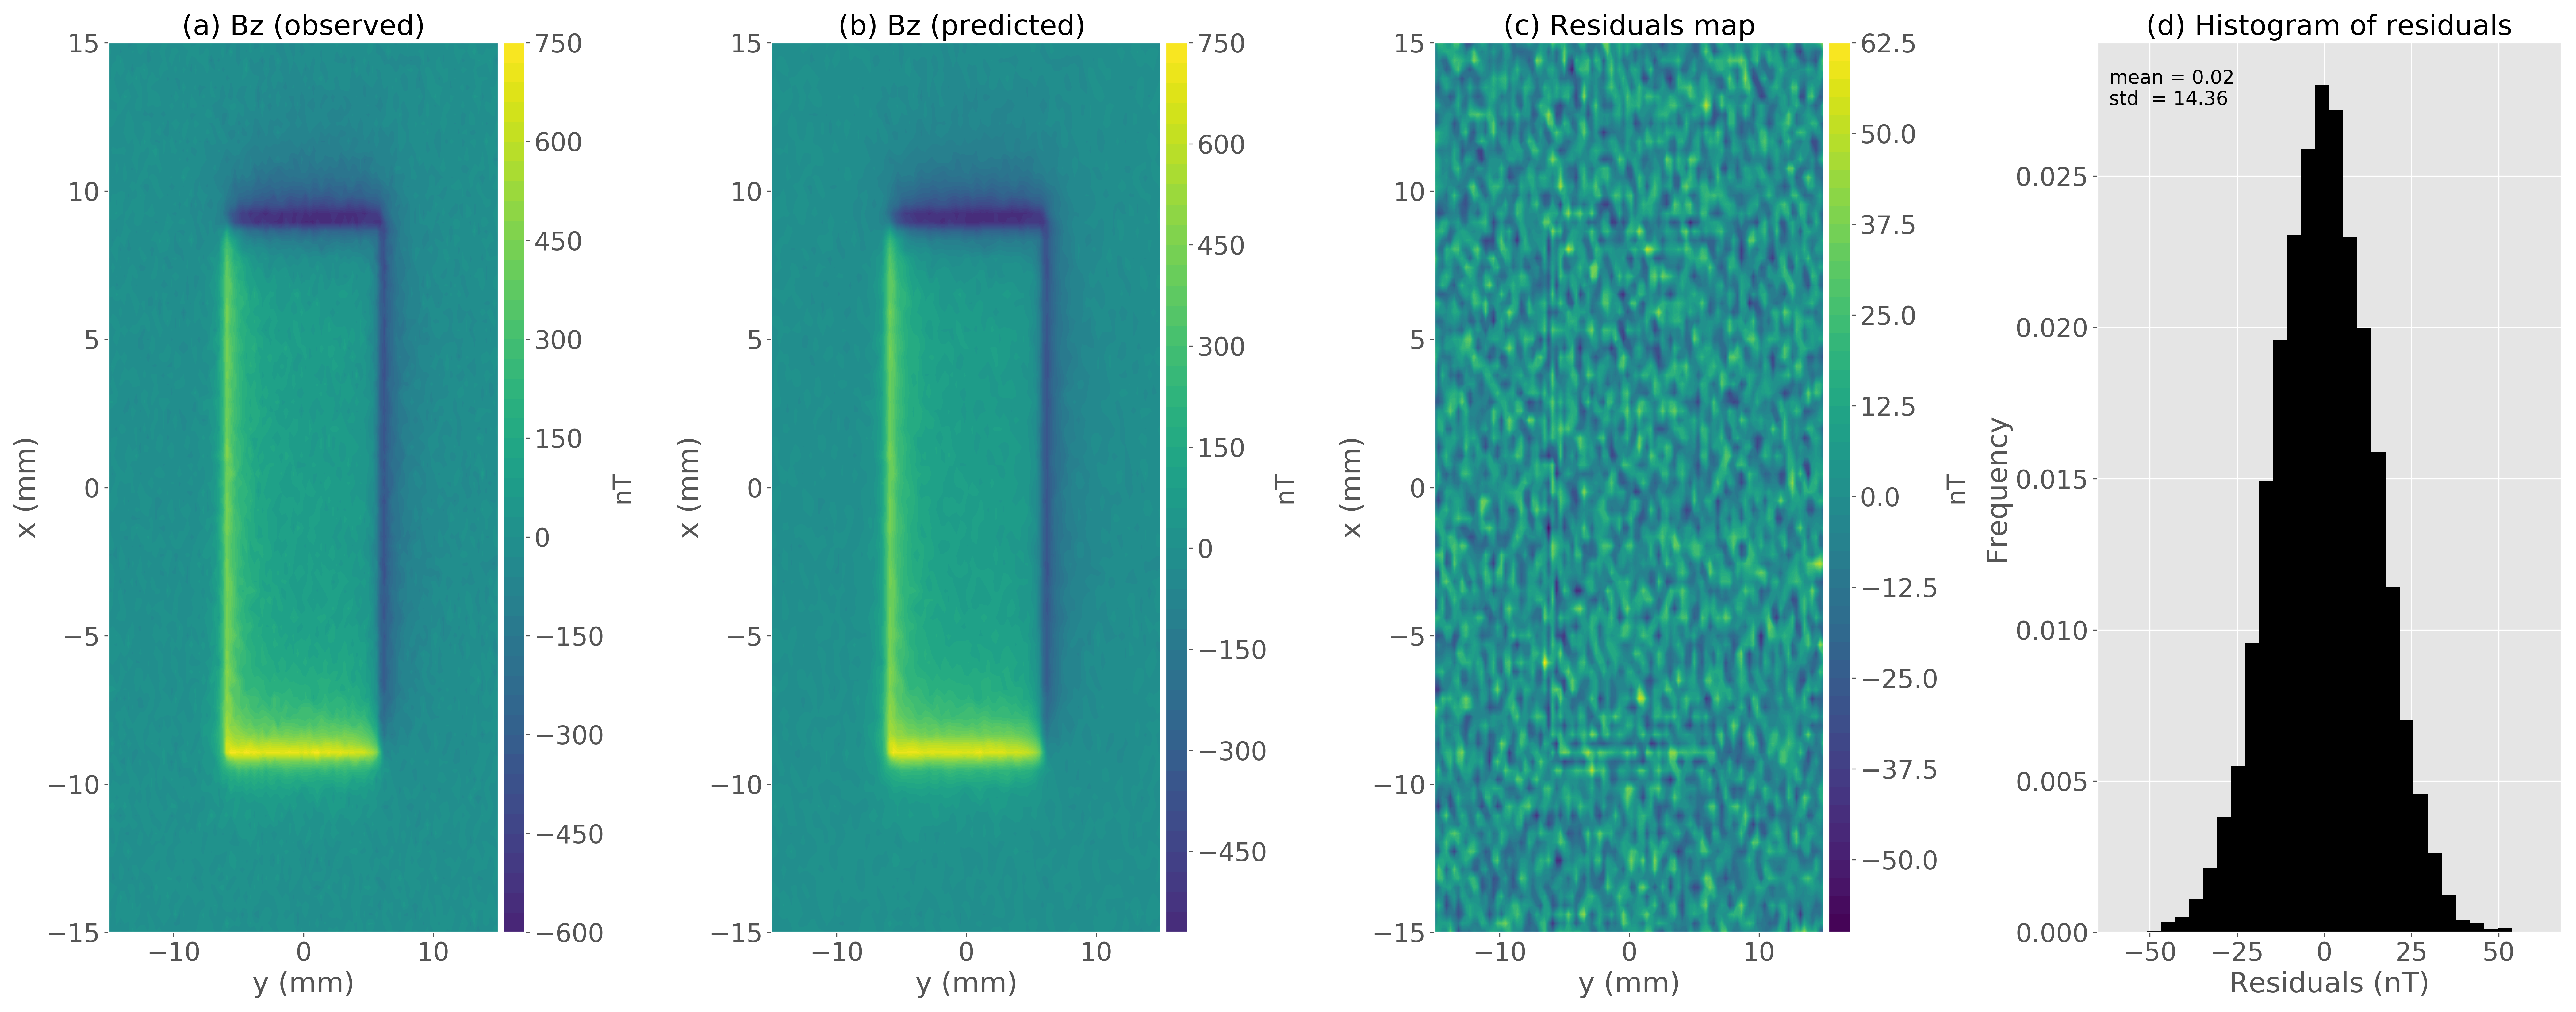
\includegraphics[width=.9\textwidth]{Fig/mag_vec/amostra_homo_correto/results_data_fitting_Bz.png}
	\caption{Aplicação a dados sintéticos para a amostra homogênea com a mesma direção de magnetização da camada equivalente. (a) Componente vertical observada. (b) Dados preditos produzido pela camada equivalente. (c) Diferença entre os dados mostrados nos gráficos a e b. (d) Histograma dos resíduos.}
	\label{fig:datafit_homo_sample_samedir}
\end{figure}

\begin{figure}
	\centering
	\includegraphics[width=1.\textwidth]{Fig/mag_vec/amostra_homo_correto/field_components_eqlayer.png}
	\caption{Aplicação a dados sintéticos para a amostra homogênea com a mesma direção de magnetização da camada equivalente. (a) Componente vertical predita pela camada. (b) Componente $x$ do campo magnético predita pela camada. (c) Componente $y$ do campo magnético predita pela camada. (d) Amplitude do campo magnético calculado através da equação \ref{eq:amplitude_field}.}
	\label{fig:components_homo_sample_samedir}
\end{figure}

\begin{figure}
	\centering
	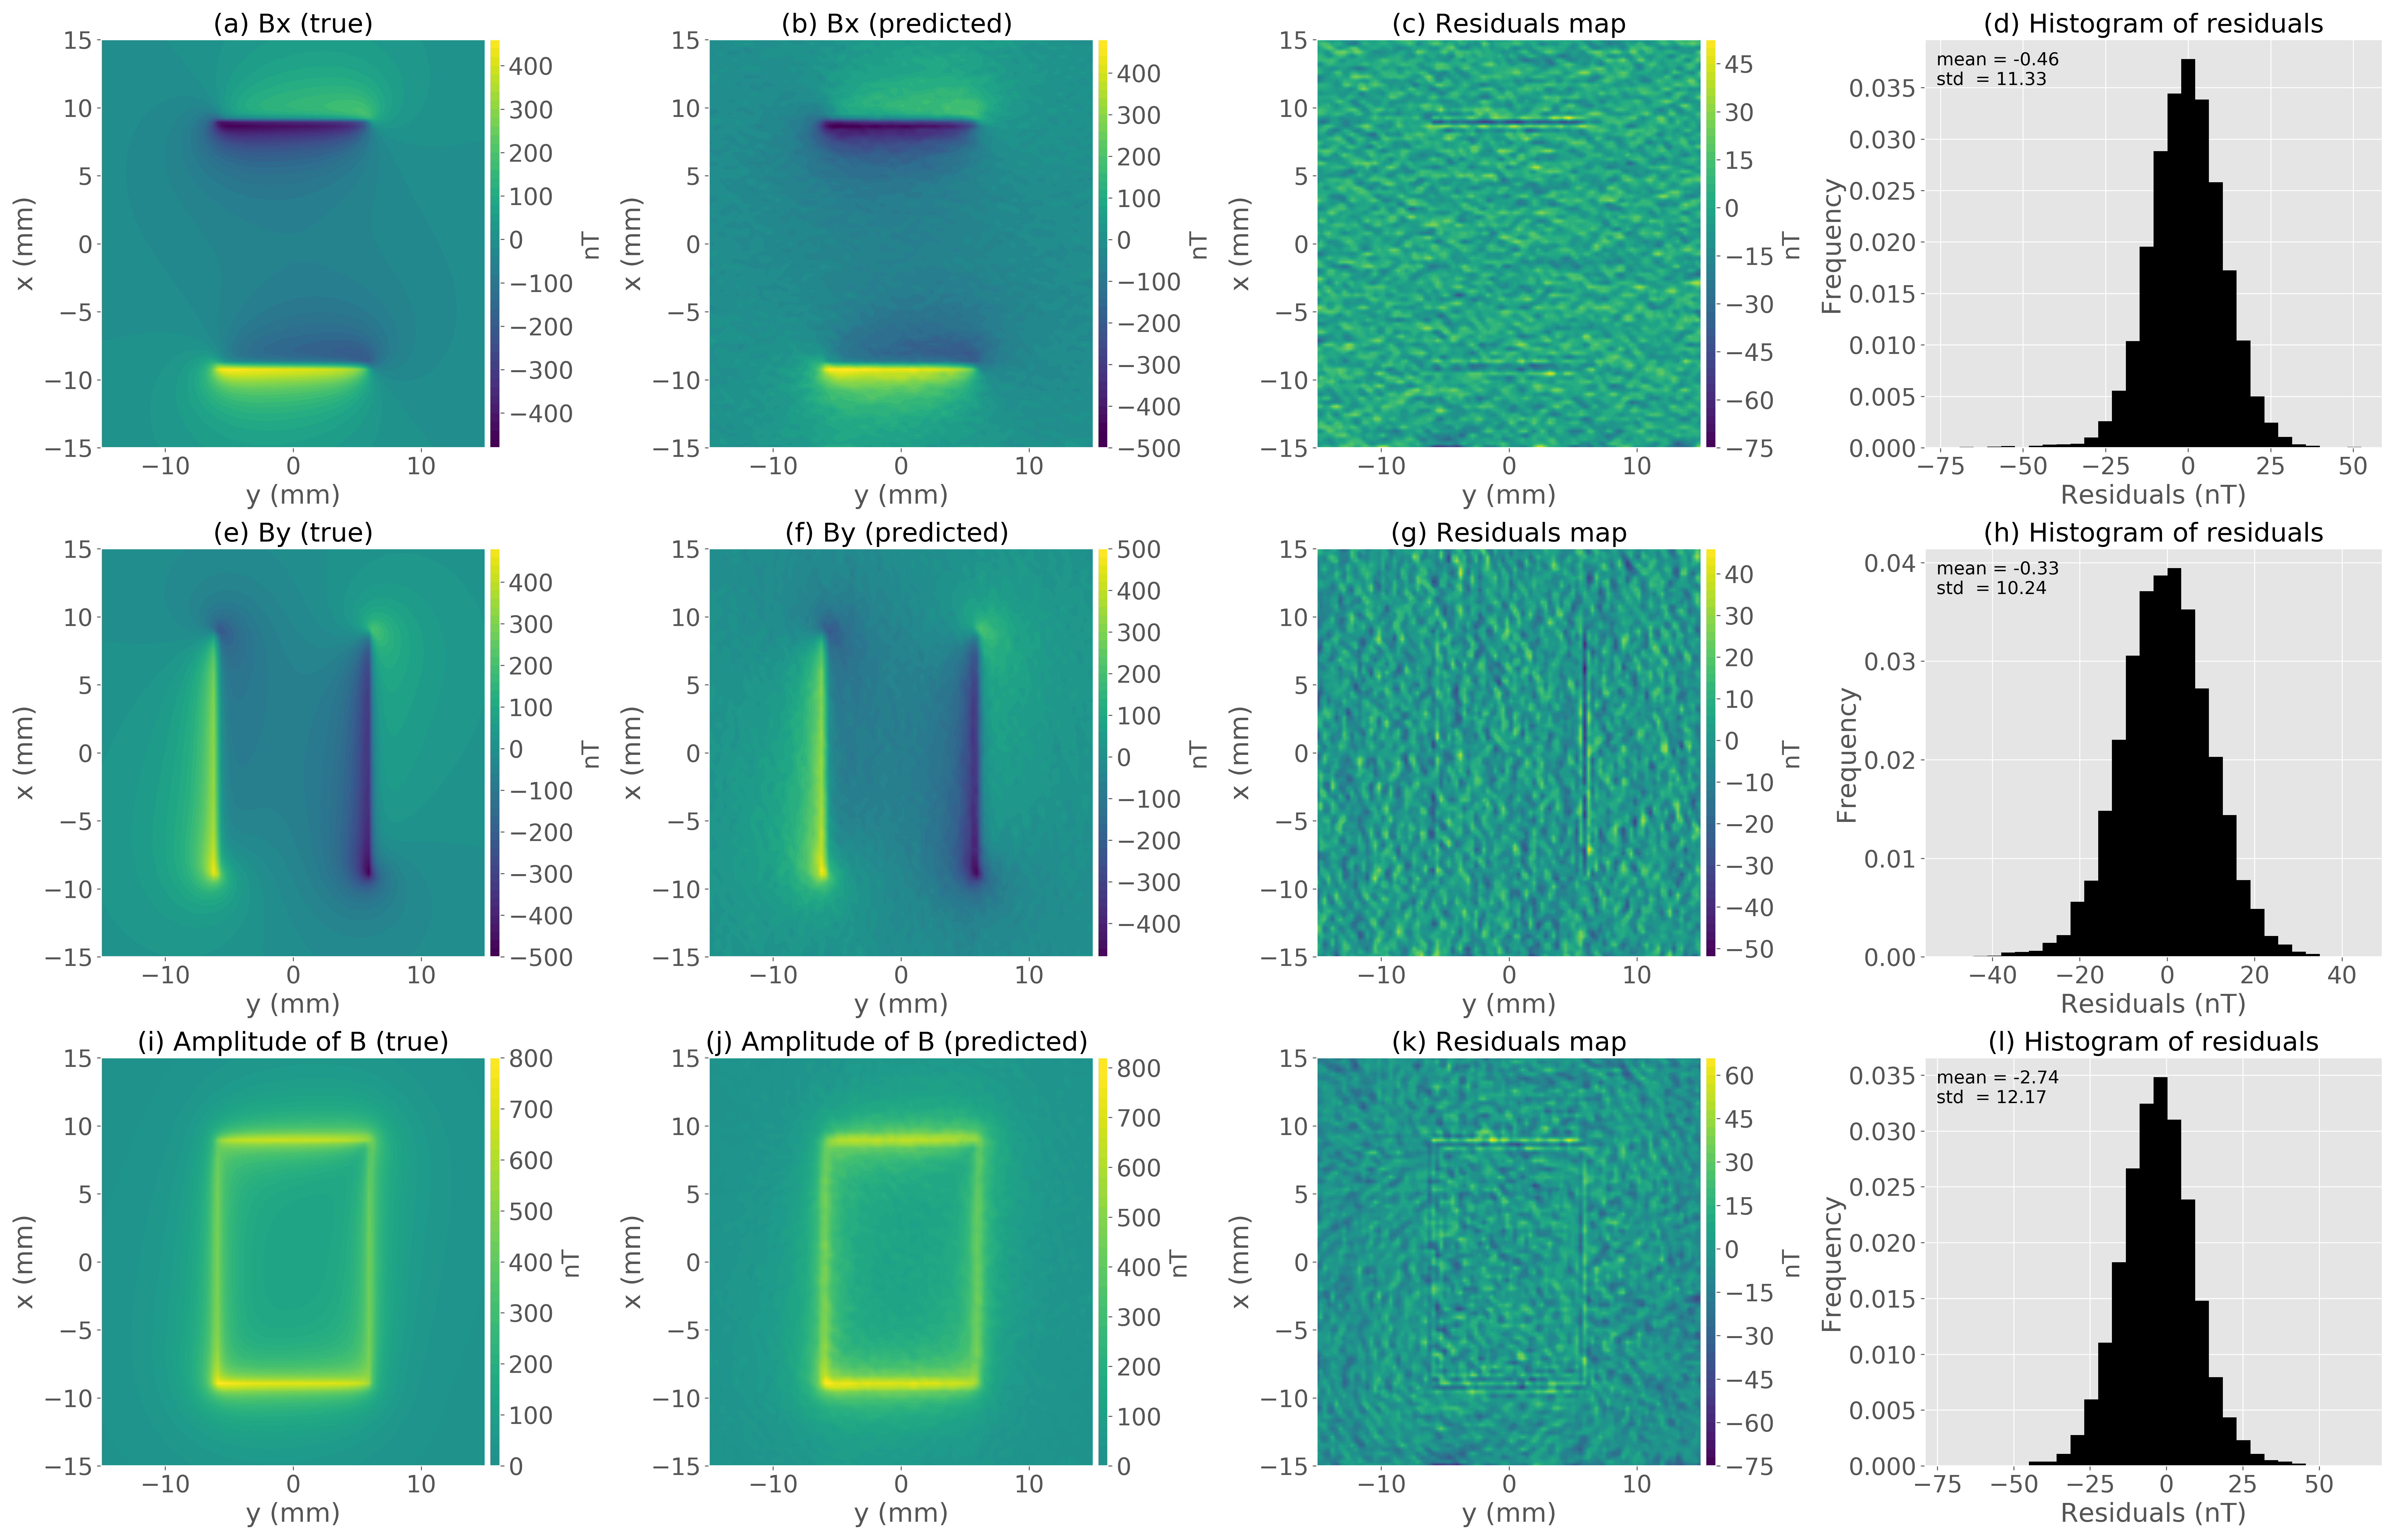
\includegraphics[width=1.15\textwidth]{Fig/mag_vec/amostra_homo_correto/comparison_true_estimated.png}
	\caption{Aplicação a dados sintéticos para a amostra homogênea com a mesma direção de magnetização da camada equivalente. (a),(e) e (i) Componentes $x$, $y$ e a amplitude verdadeiras do campo magnético, respectivamente. (b), (f) e (j) Componentes $x$, $y$ e a amplitude do campo magnético preditas pela camada equivalente, respectivamente. (c), (g) e (k) Mapas dos resíduos. (d), (h) e (l) Histograma dos resíduos.}
	\label{fig:comparison_homo_sample_samedir}
\end{figure}


\subsection{Camada equivalente com direção de magnetização diferente da amostra}
\label{subsec:homo_dif_dir}

Utilizamos uma camada equivalente composta por um grid de $100 \times 100$ posicionados a uma profundidade de $z_c = 750$ microns abaixo do plano de observação. A direção de magnetização para as fontes equivalente foi de $50^\circ$ para a inclinação e $60^\circ$ para a declinação, enquanto a amostra possui $20^\circ$ para a inclinação e $30^\circ$ para a declinação. Utilizando a equação \ref{eq:linear_sys_p_z}, estimamos a distribuição de momentos magnéticos (não mostrado). A figura \ref{fig:datafit_homo_sample_difdir}b mostra os dados preditos produzidos pela camada equivalente. A figura \ref{fig:datafit_homo_sample_difdir}c mostra os resíduos definidos pela diferença entre os dados simulados (Figura \ref{fig:datafit_homo_sample_difdir}a) e os dados preditos (Figura \ref{fig:datafit_homo_sample_difdir}b). Os resíduos aparecem com distribuição normal de média $-0,02 \, nT$ e desvio padrão $15,02 \, nT$ como mostrado na figura \ref{fig:datafit_homo_sample_difdir}d. Com a distribuição de momentos magnéticos estimada, conseguimos calcular as componentes e a amplitude do campo magnético através das equações \ref{eq:pred_vec_x}, \ref{eq:pred_vec_y} e \ref{eq:amplitude_field} (Figura \ref{fig:components_homo_sample_difdir}a-d). Com o objetivo de verificarmos se a camada equivalente produziu as componentes e a ampĺitude do campo magnético com sucesso, calculamos os valores verdadeiros que são mostrados nas  figuras \ref{fig:comparison_homo_sample_difdir}a, \ref{fig:comparison_homo_sample_difdir}e e \ref{fig:comparison_homo_sample_difdir}i. As figuras \ref{fig:comparison_homo_sample_difdir}b, \ref{fig:comparison_homo_sample_difdir}f e \ref{fig:comparison_homo_sample_difdir}j são os dados preditos pela camada equivalente. As figuras \ref{fig:comparison_homo_sample_difdir}c, \ref{fig:comparison_homo_sample_difdir}g e \ref{fig:comparison_homo_sample_difdir}k são resíduos entre os dados verdadeiros e os dados preditos pela camada. As figuras \ref{fig:comparison_homo_sample_difdir}d, \ref{fig:comparison_homo_sample_difdir}h e \ref{fig:comparison_homo_sample_difdir}l são os histogramas dos resíduos. Os resultados mostram que apesar da camada equivalente ter direção de magnetização muito diferente da direção da amostra, as estimativas para as componentes e a amplitude do campo magnético foram aceitáveis.  

%%% Figuras 

\begin{figure}
	\centering
	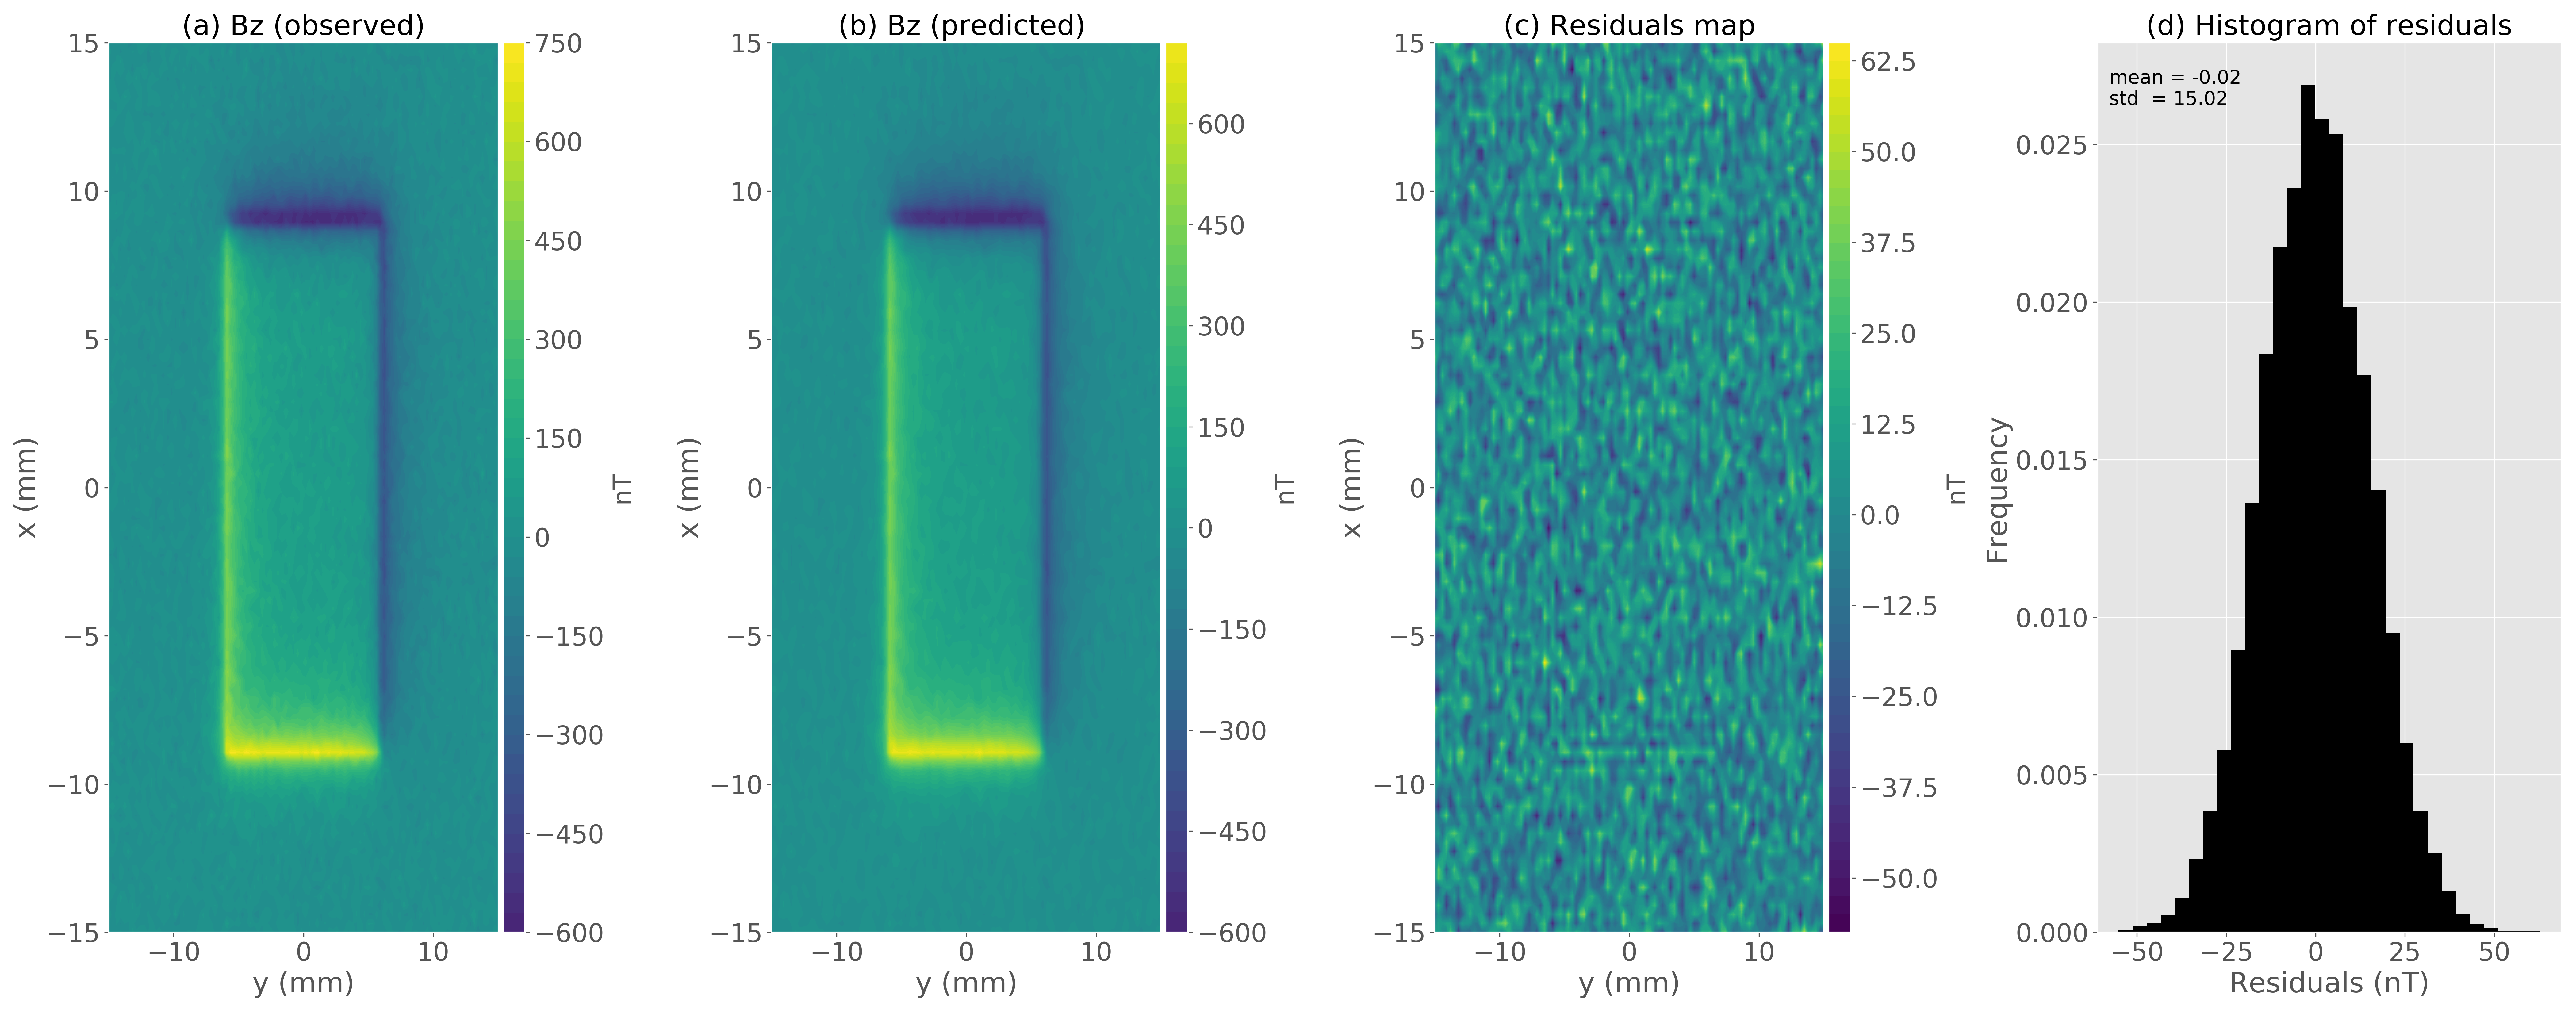
\includegraphics[width=.9\textwidth]{Fig/mag_vec/amostra_homo_errado/results_data_fitting_Bz.png}
	\caption{Aplicação a dados sintéticos para a amostra homogênea com direção de magnetização diferente da camada equivalente. (a) Componente vertical observada. (b) Dados preditos produzido pela camada equivalente. (c) Diferença entre os dados mostrados nos gráficos a e b. (d) Histograma dos resíduos.}
	\label{fig:datafit_homo_sample_difdir}
\end{figure}

\begin{figure}
	\centering
	\includegraphics[width=1.\textwidth]{Fig/mag_vec/amostra_homo_errado/field_components_eqlayer.png}
	\caption{Aplicação a dados sintéticos para a amostra homogênea com direção de magnetização diferente da camada equivalente. (a) Componente vertical predita pela camada. (b) Componente $x$ do campo magnético predita pela camada. (c) Componente $y$ do campo magnético predita pela camada. (d) Amplitude do campo magnético calculado através da equação \ref{eq:amplitude_field}.}
	\label{fig:components_homo_sample_difdir}
\end{figure}

\begin{figure}
	\centering
	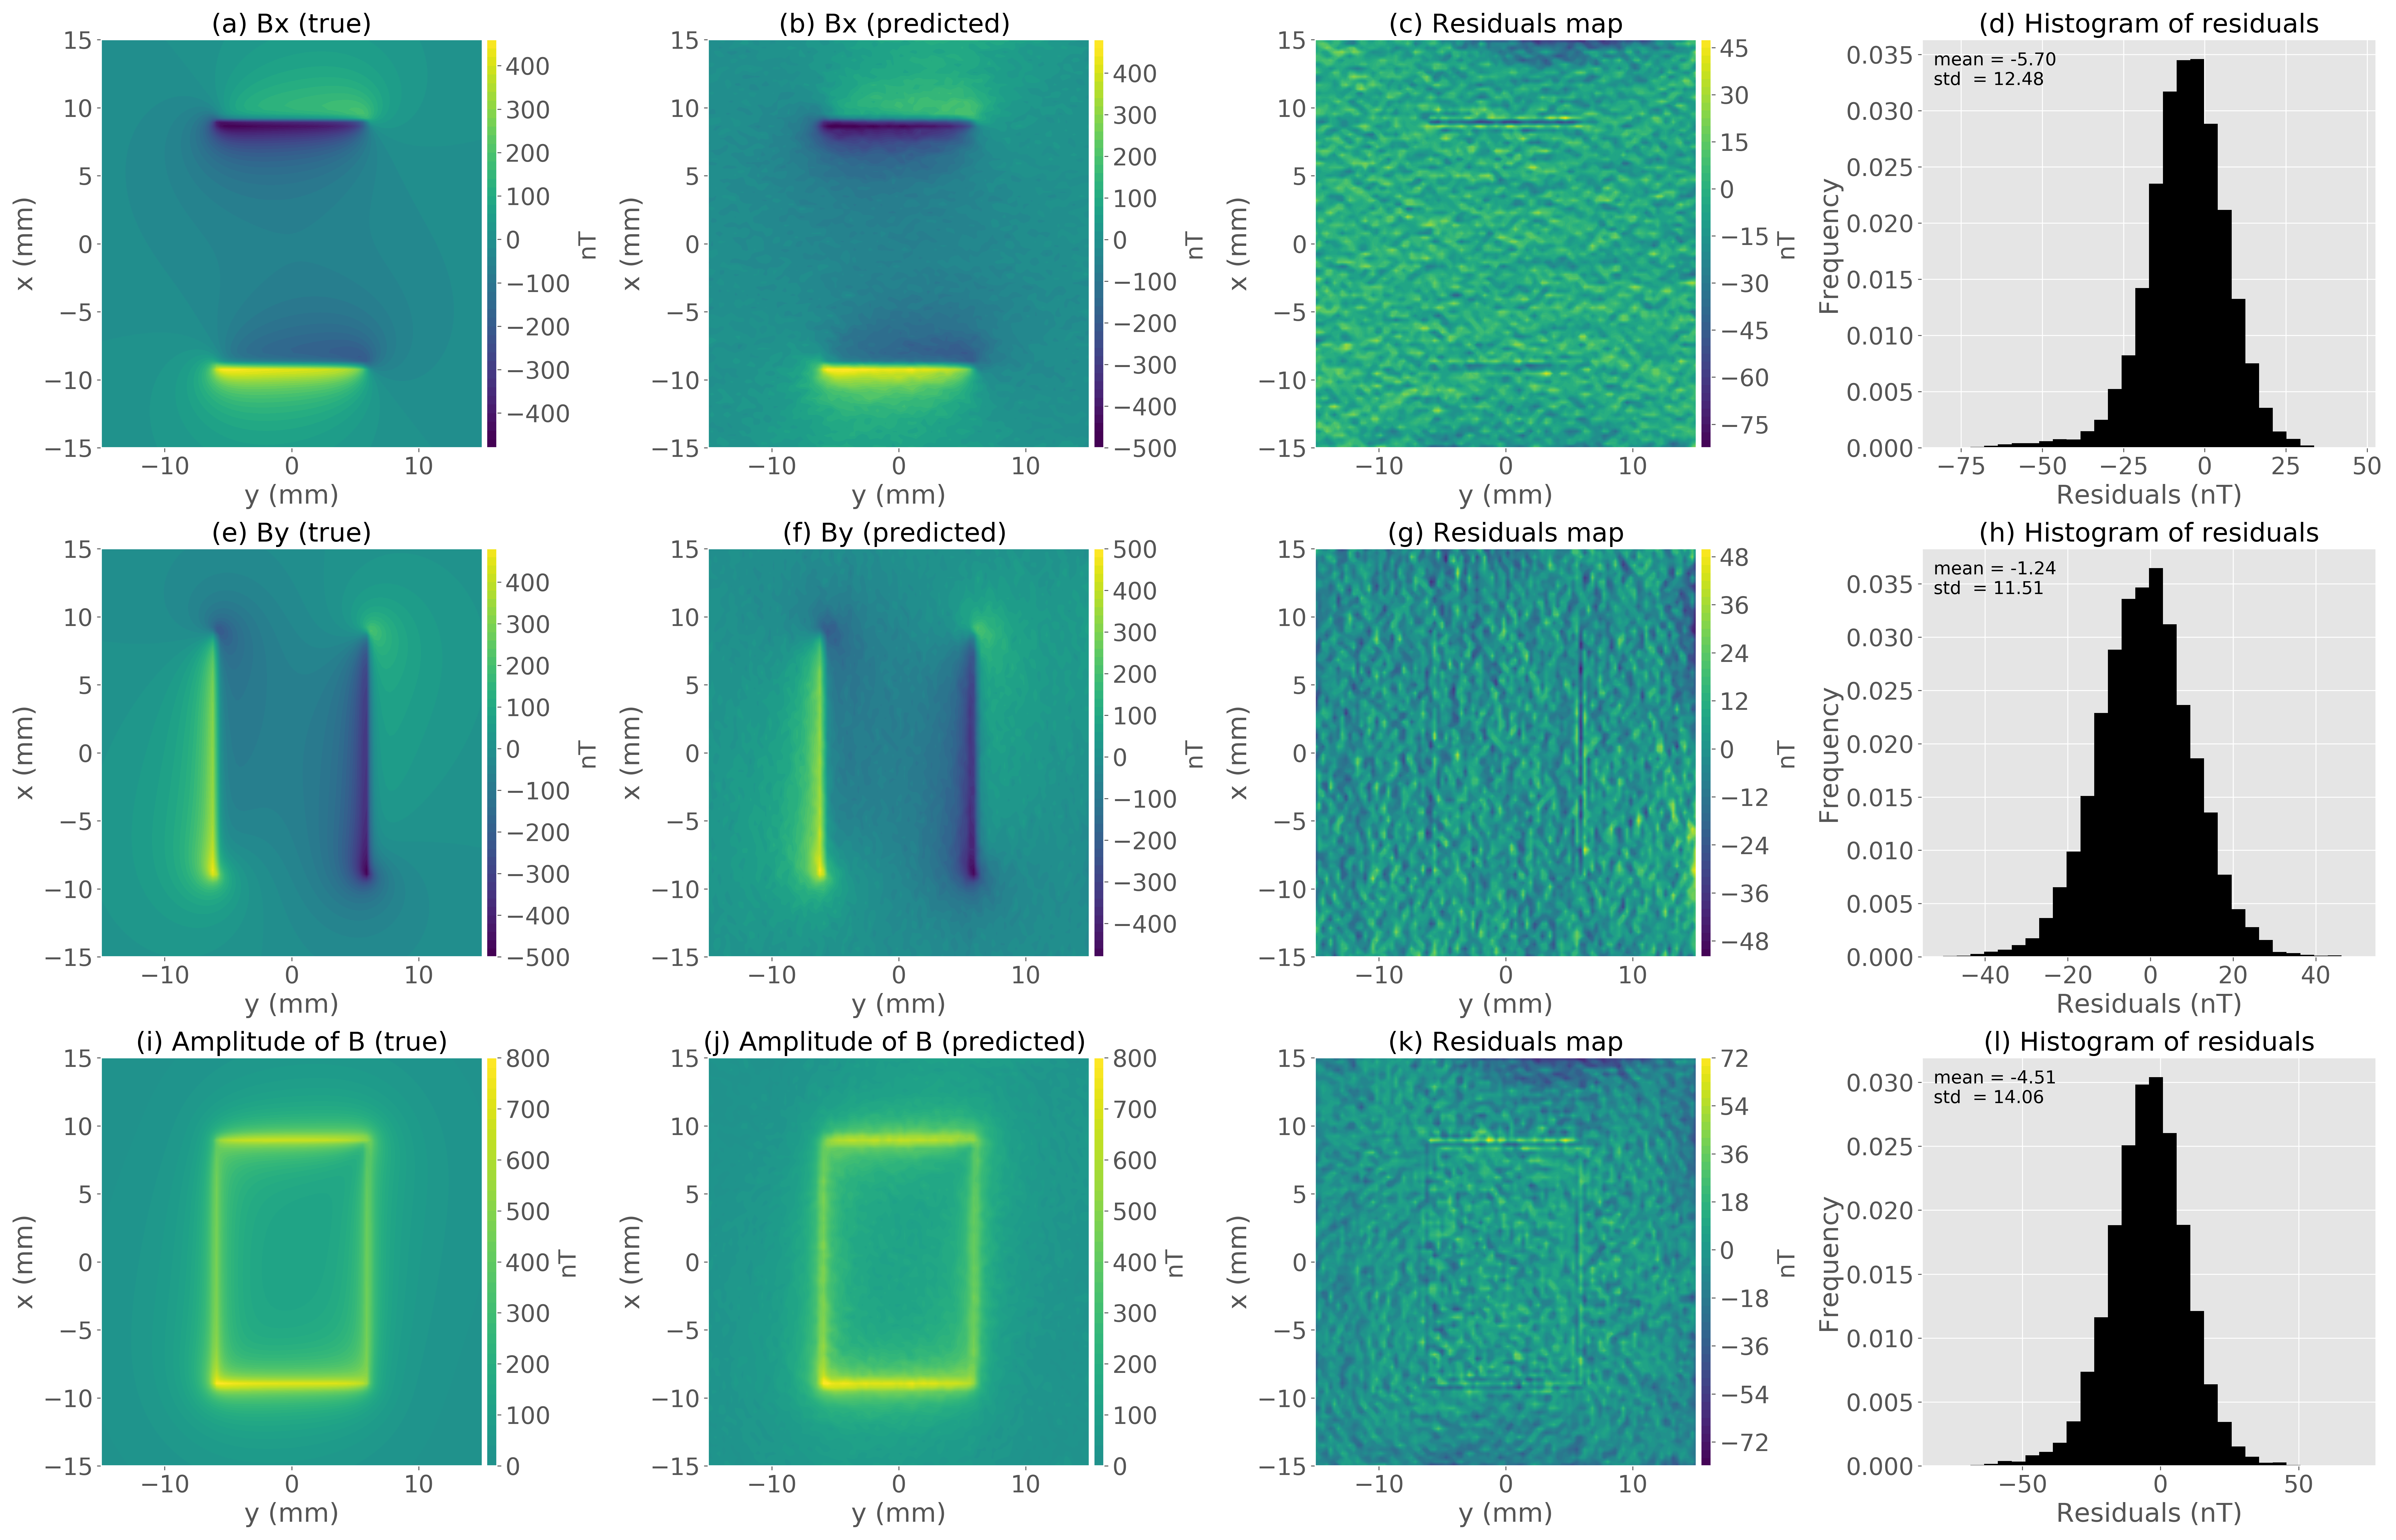
\includegraphics[width=1.15\textwidth]{Fig/mag_vec/amostra_homo_errado/comparison_true_estimated.png}
	\caption{Aplicação a dados sintéticos para a amostra homogênea com direção de magnetização diferente da camada equivalente. (a),(e) e (i) Componentes $x$, $y$ e a amplitude verdadeiras do campo magnético, respectivamente. (b), (f) e (j) Componentes $x$, $y$ e a amplitude do campo magnético preditas pela camada equivalente, respectivamente. (c), (g) e (k) Mapas dos resíduos. (d), (h) e (l) Histograma dos resíduos.}
	\label{fig:comparison_homo_sample_difdir}
\end{figure}


%%%%%%%%%%%%%%%%%%%%%%%%%%%%%%%%%%%%%%%%%%%%%%%%%%%%%%%%%%%%%%%%%%%%%
\section{Simulação de amostra com heterogeneidades}
\label{sec:hetero_sample}
